\subsection{Interaction}
A QActor can interact with others (local or remote) QActor by sending/receiving messages. A QActor can also emit or sense events. Here it is a schema of all the interactions occurring between the different contexts defined previously in the Structure subsection.
\begin{figure}[h]
	\centering
	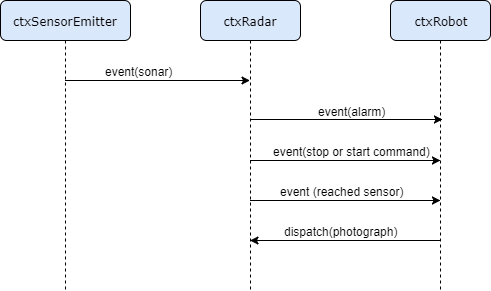
\includegraphics[width=\linewidth]{interaction.png}
	\caption{Interactions between the three contexts.}
\end{figure}